\part{Introduction}

An embedded system is a combination of hardware and software components put together to achieve a specific task. Often, embedded systems are built into a larger device or system and are used to collect, store, process, and analyse data, as well as to control the device\textquotesingle s behaviour. Embedded devices are a category of tiny devices with physical, computational and memory constraints that are programmable to perform dedicated tasks.

Like most of the automotive industry, Scania employs embedded systems called Electronic Control Units (ECUs) in their trucks to supervise and regulate essential subsystems like the engine, transmission, braking, and electrical systems. Each of these subsystems has one or more ECUs to gather system data and transmit it to a central communicator where the data is processed and the systems operations are monitored.

Scania currently runs a massive fleet of around 600,000 connected heavy vehicles. The company's truck sales make up 62\% of its global sales and Scania has been adding 60,000 trucks to it's fleet annually \cite{scania-report}. This large fleet of rolling vehicles that are connected though the communicators opens up new possibilities. These connected devices continuously monitor the state of the vehicle and this data can be used to accurately
and efficiently schedule vehicle maintainance. For example, if a tire change is predicted to be required in 100 kms then the driver can plan the route smartly to reach the workshop before the vehicle breaks down. This opportunity can be realised by running smart algorithms on the hardware that is currently available.

Machine learning (ML) on embedded devices is becoming increasingly popular due to its ability to provide real-time insight and intelligence to devices. This technology can be used to automate tasks, improve efficiency, and make better decisions. But this technology presents a unique set of challenges due to the limited resources available on these devices. Embedded devices are designed to be power efficient, have limited memory and processing power, and require closely tailored algorithms, making it difficult to use pre-existing machine learning models. Furthermore, embedded devices are often expected to produce real-time results, which further complicates the development process. Despite these challenges, machine learning on embedded devices has potential applications in a variety of areas, such as in the fields of robotics and autonomous vehicles.

One such ML application Scania has been developing in their \textsc{LOBSTR} \cite{lobstr} and \textsc{FAMOUS} \cite{famous} projects is the anomaly and fault detection models in a federated learning environment. Targeting to run the anomaly detection models on the existing ECUs with limited resources has many benefits and challenges.

\subsection*{Benefits to performing Anomaly Detection on ECUs}

\begin{itemize}
	\item Scania is committed to promote a shift towards autonomous and eco-friendly transport systems. The latest addition of Scania's connected trucks and buses will be embedded with upgraded ECUs and communication devices. However, this upgrade will make the stock of older hardware devices to become obsolete and regarded as e-waste, which could be prevented. Exploring the possibility of repurposing existing ECUs to run ML models aligns with Scania's vision of leading the way towards a sustainable future.
	\item Neural networks (NNs) are a type of machine learning that can detect intricate patterns not only across multiple data signals but also over time. \textit{include benefits to NN approach to Anomaly Detection}
	%Achieving this level of performance is computationally demanding, and training NNs on embedded devices requires careful resource management. However, being able to efficiently train NNs on embedded devices with high accuracy could unlock significant potential for future advancements. (could include benefits of NN for anomaly detection)
	\item Federated learning methods facilitate the training of pre-trained anomaly detection models on the ECUs installed in Scania's distributed fleet of connected trucks. Each ECU individually trains the model with its data and transmits the updated model parameters to a central server. This distributed learning approach enables early detection of faults or failures and ensures that critical data remains on the device. Also dependency on network bandwidth is reduced as only the aggregated model updates are communicated over the network, instead of transmitting the entire data sample.
\end{itemize}

\subsection*{Challenges to implementing Federated Models}

\begin{itemize}
	\item To reap the best benefits of these approaches, training of the model needs to be performed on board. However much of the potential of running machine learning applications on these devices remains unattained due to the difficulties in creating these applications and running training on-board. Approaches such as TensorFlow Lite (TFLite), Edge Impulse, and STM Cube AI implemented along the TinyML frameworks, enable running ML models targeted for small resource devices. However these approaches are largely limited to inference capabilities and there is no adequate open source support in the existing infrastructure for training ML models.
	\item An Original Equipment Manufacturer (OEM) is responsible for the development and upkeep of the Scania ECU. However, the amount of information made available regarding the hardware design, memory layout, and operating system (OS) is restricted. To construct an embedded OS for a customized hardware, critical details such as the device tree, memory organisation, and boot flow are necessary. Obtaining this information from a functional board can be an enormous task requiring reverse engineering expertise.
\end{itemize}

% Reason :
	% 1. Sustainabililty - check
	% 2. Potential in tiny ML (billions of devices) and Federated Learning approaches
			% Needs Training on board

% Gap  in the market: No support for training ML models on embedded devices
% Scope: Exploring the challenges of building and training NN's on embedded devices using different approaches and evaluating their performances.
% TODO: Attach a reference for the following claim

%Among the ML approaches to take, Artifical Neural Networks are especially interesting for anomaly detection due to several factors such as minimal data preprocessing \dots To get the best out of this approache, training of the model needs to be performed on-board. However much of the potential of running machine learning applications on these devices remain unattained due to the difficulties in creating these applications and running training on-board.

\subsubsection{Problem Description}
The scope of the thesis is to repurpose the existing Scania ECU and explore the challenges of building targeted NN models and training them on repurposed ECU using different approaches and evaluating their performances.

%The scope of the thesis is to explore the challenges of building and training neural networks on embedded devices using different approaches and evaluating their performance.

%An important feature of machine learning applications are their iterative improvement process. For neural network applications this happens during the training process which traditionally consumes a lot of compute resource

% \subsubsection{Why perform training and inference on ECUs?}

% In the world of embedded systems resources such as compute, memory, network bandwith etc. are all limited. The traditional model of sending data from embedded device sensors off-board to compute clusters on the cloud presents several challenges such as bandwith consumption, privacy considerations, and more that makes it attractive to perform both training and inference on-board the embedded device

% \paragraph{Federated Learning}{
% 	One approach to making this training loop take place from within these platforms is Federated Learning which cruicially allows for the data to remain on the device
% }

\chapter{Background}

Developing and maintaining applications that rely on neural network models on a fleet of embedded devices has several considerations. The application deployment process should allow for continuous updates to the neural network, transfer data or model updates from the embedded devices to off-board analytics or machine learnining pipelines, and not interfere with the other applications on the embedded device, all the while maintaining correct representations in the neural network model. It is thus important to have an operating system that can support these applications with features such as process isolation, inter process communication mechanisms, multitasking etc.

The target embedded device to run these applications are the ECUs aboard a Scania vehicle. These ECUs have application processor cores that are capable of running rich operating systems such as linux distributions or real-time operating systems such as QNX, or VxWorks. All these operating systems also support hypervisors which allows for configurations where a host operating system runs standard automotive applications in addition to a guest operating system running the neural network application. This approach has the advantage of mitigating application crashes in the guest operating system and can provide a level of protection against software vulnerabilities \cite{linux-guest-os}. Linux is the prefered choice for such a guest operating system due to its configurability and rich support for application development.

The next section looks at developing such an embedded linux environment and the process of developing neural network applications for that operating system.

\section[Development Process for Embedded Linux]{Development For Embedded Linux}

Building and maintaining embedded linux distributions with linux kernel and user mode applications require tools that can provide build configuration support at multiple levels, build a cross compiling toolchain or interface with one, support for several \verb!C! run times, and provide support for project management. There are several tools that provide this support such as OpenADK, The Yocto project, Buildroot, OpenWrt, etc. Out of them Yocto and Buildroot are the most widely used and most featureful.

\subsection[SDKs \& Compiler Toolchains]{Toolchains \& Cross compilers}

Creating applications that are to be run on an embedded devices requires a set of software components that are usually collectively referred to as Software Development Kits (SDK). This suite of programs usually contain a toolchain that is capable of converting application source code, such as those in \verb!C!  or \verb!C++! , into executables that can be run on the target embedded device.

Software development toolchains consists of a compiler, linker, libraries, debuggers, etc., to create and manage executable binary programs for a target device - the most common one being GNU binary utilities, a.k.a binutils. The primary choice for \verb!C! compilers in this list of utility programs is GCC, with LLVM's Clang being another alternative. For developing applications that interface with the linux operating system APIs the toolchain also produces necessary header files called linux kernel header files. The last important piece of a toolchain will be the \verb!C! runtime, with the most popular choice being GNU's glibc.

Building an embedded linux kernel requires several configuration parameters describing the kernel configuration, enabled feature, and more. To port linux onto a process on a particular board requires creating a boot loader capable of that task as well. A boot loader program is responsible for placing an operating system into memory. This process will also need to be supported by the build system configurations. The majority of the details as to how the boot loader has to be configured will be based on the pariticular hardware that it will be configured for.

Supporting embedded hardware requires a software stack that includes several components such as the bootloader, the root file system, and the operating system. The initial target machine was an ECU filling the role of a communicator on the truck. Certain support components for this board are unavailable, such as the Yocto meta layer used for the existing software on board, memory mapping for the attached devices, source codes for boot ROM firmware or the boot loader, etc. The reverse engineering efforts to attain this information were dropped due to time constraints and ultimately a similiar board, namely the iMX6SDB evaluation board, with the required information publicly provided by processor chip vendor NXP was chosen as the target platform. The details of the attempt at uncovering this information is layed out in \hyperref[rtc-c300]{Appendix II}.

\subsection{Developing using QEMU}

\section{Neural Network Application Development}

In general, neural network applications are written using machine learning frameworks or software libraries meant for scientific computing. The machine learning frameworks themselves are build on top of multiple software libraries meant for specific aspects of machine learning calculations. Several libraries exist that target specific subproblems in such computations and provide optimised implementations of several different processor architectures.

\subsection{Choice of Software Stacks and Programming Languages}

As most neural network applications are written in frameworks like PyTorch and Tensorflow, they have thriving ecosystems that provide rich developer support. Machine learning based companies and their service offerings such as cloud machine learning platforms almost invariably targets these platforms and provide several software tools for developers to utilize. Developers in these platforms enjoy several resources such as productivity tools that allows for continuous integration and development, maintainance and other resources with features for performance profiling, debugging, orchestration, etc. ML and neural network service provides always target for these frameworks in their produces.

Another aspect to consider is the programming language in which the neural network will be written up in. Most machine learning models at present are written in Python and frameworks like PyTorch and Tensorflow have richer interfaces for Python compared to other programming languages. This is unfavourable to embedded devices where a Python application may take up higher memory and have longer latencies. The programming language of choice for embedded applications however is \verb!C! and \verb!C++! which are supported by the ML frameworks but not to the same extent as their Python interfaces.

\subsection{Embedded Software Stacks for Neural Networks}

One complication caused by relying on software stack of the manner discribed before is software bloat. This causes a bigger problem in the context of embedded devices where resources are limited. There has been significant efforts made to clear this concern for the world of embedded devices, especially motivated by interests in getting neural network applications ready for mobile devices

\section{Training on Device}

The traditional model for machine learning applications on embedded devices

\begin{center}
	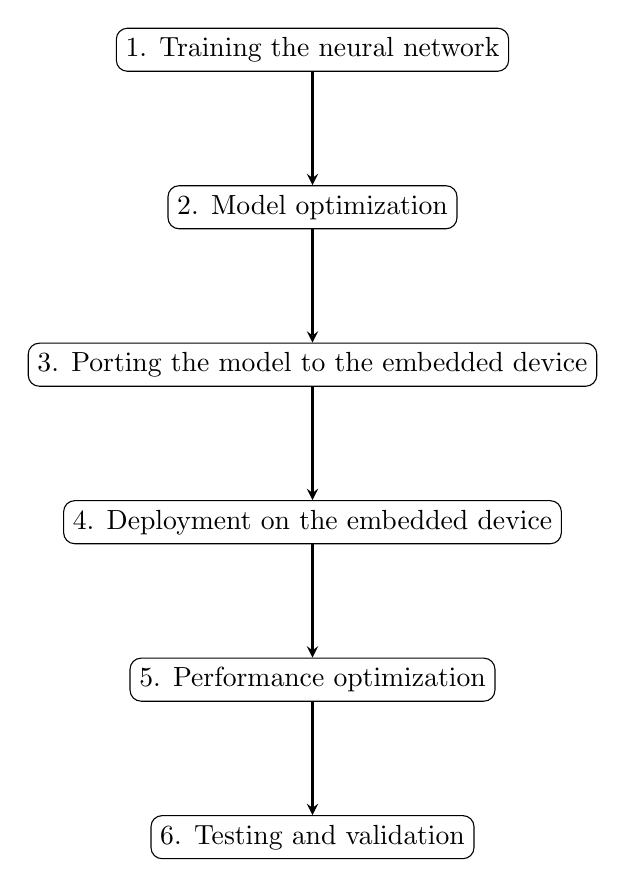
\begin{tikzpicture}[node distance=2cm, every node/.style={rectangle, draw, align=center, rounded corners}, arrow/.style={->, >=stealth, thick}]
	\node (train) {1. Training the neural network};
	\node (optimize) [below of=train] {2. Model optimization};
	\node (port) [below of=optimize] {3. Porting the model\ to the embedded device};
	\node (deploy) [below of=port] {4. Deployment on the embedded device};
	\node (perf-opt) [below of=deploy] {5. Performance optimization};
	\node (test) [below of=perf-opt] {6. Testing and validation};

	\draw [arrow] (train) -- (optimize);
	\draw [arrow] (optimize) -- (port);
	\draw [arrow] (port) -- (deploy);
	\draw [arrow] (deploy) -- (perf-opt);
	\draw [arrow] (perf-opt) -- (test);

	\end{tikzpicture}
\end{center}

\subsection{Federated Learning}

Federated learning is a technique of training ML models in a distributed way, where each client or device uses its own data set to train a local model. A client application on a truck generates sensor data created by the operation of the vehicle. Each vehicle then trains on-board a local model which is then centrally collected and aggregated to build a global model. This global model can then be used for inference in each client. In the LOBSTR \cite{lobstr} and FAMOUS \cite{famous} projects Scania has developed statistical models and NN models for anomaly detection. The statistical models are lightweight and can easily be trained with limited computational resources. These neural network models are computationally heavy and hard to train with limited resources. The existing ECUs are not tailored for ML and general purpose ML frameworks often are hard to use in this embedded systems, specially for training purposes.

This thesis focuses on repurposing existing hardwared (ECU) to ML edge devices that are tailored to train NN in the most efficient possible way. We try to reverse engineer the old communicator model to build a custom Yocto project tailored for ML. As alternative test ECU we use an evaluation board that has similar specifications as the commuicator to benchamark and experiment different NN implementations and evauluate the optimal ones.

\chapter{Theory}

In the following section an overview of the nature of computations involved in neural network applications is presented. Afterwards introductions are made to some terminology associated with software development for embedded devices, contextualised in embedded linux and its application development. The final section gives a short overview of conducting application performance evaluation.

\section{Neural Networks}

Training a machine learning model is fundamentally computing several floating point multiply and accumulate operations.

\section{Embedded Linux Environment}

As described in the previous chapter, embedded linux and user mode applications are using embedded build systems such as Buildroot or Yocto.

\subsection{A Simplified Embedded Boot Sequence}

\section{Performance Evaluation}

Roofline model for a simple matrix multiply application on Cortex-A9
